\documentclass[11pt]{ctexart}
\usepackage[a4paper,margin=1in]{geometry}
\usepackage{amsmath}
\usepackage{amssymb}
\usepackage{booktabs}
\usepackage{graphicx}
\usepackage{tikz}
\usepackage{xcolor}
\usepackage{listings}
\usepackage{float}
\usepackage{longtable}
\usepackage{array}
\usepackage{caption}
\usepackage{setspace}

\onehalfspacing
\setlength{\parindent}{2em}
\setlength{\parskip}{0.4em}

\lstdefinelanguage{TLA}{
  morekeywords={MODULE,EXTENDS,CONSTANT,CONSTANTS,VARIABLES,ASSUME,Init,Next,Spec,TypeOK,THEOREM},
  sensitive=true,
  morecomment=[l]{\\*},
  morestring=[b]"
}

\lstset{
  basicstyle=\ttfamily\small,
  keywordstyle=\color{black},
  commentstyle=\color{black},
  stringstyle=\color{black},
  breaklines=true,
  frame=single,
  columns=fullflexible
}

\title{\textbf{基于 TLA+ 的弱二元信号量互斥协议验证}\\CE356 课程项目最终报告}
\author{Tianbin Wang \and Kehao Zhang}
\date{2026 年 6 月}

\newcommand{\growthlegendbox}{%
\fbox{%
\begin{tabular}{@{}c@{\hspace{0.4em}}c@{\hspace{1.2em}}c@{\hspace{0.4em}}c@{}}
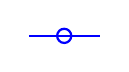
\begin{tikzpicture}[baseline=-0.6ex]
\draw[blue, thick] (0,0) -- (0.9,0);
\draw[blue, thick] (0.45,0) circle (0.09);
\end{tikzpicture}
& Baseline
&
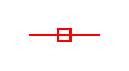
\begin{tikzpicture}[baseline=-0.6ex]
\draw[red, thick] (0,0) -- (0.9,0);
\draw[red, thick] (0.37,-0.08) rectangle (0.53,0.08);
\end{tikzpicture}
& Udding
\end{tabular}}%
}

\begin{document}
\maketitle

\begin{abstract}
我们研究 CE356 课程项目中的弱二元信号量互斥问题：在只允许使用 weak binary semaphores 的条件下，实现参数化的 $n$ 进程 mutual exclusion，并用 TLA+ 说明其正确性。我们沿用 midterm 的整体思路，将项目组织为一个对照式研究：一方面，我们建立最朴素的单 \texttt{mutex} baseline，用来说明仅有互斥并不足以解决公平性问题；另一方面，我们建立 Udding 算法的 TLA+ 模型，用来刻画其针对 overtaking 和 starvation 的分阶段准入机制。我们对两个模型进行了 $n=2$ 到 $n=7$ 的 TLC 参数实验，并进一步在显式 fairness assumptions 下，对 Udding 模型的 \texttt{NoStarvation} 性质进行了小规模时序验证。结果表明，baseline 和 Udding 都满足 safety 层面的互斥性质，而 Udding 在公平性相关的 liveness 检查上也表现出与原始算法目标一致的行为，但其状态空间复杂度显著更高。
\end{abstract}

\section{引言}

课程题目要求我们：

\begin{quote}
使用 only weak binary semaphores 实现 $n$ process mutual exclusion，并用 TLA+ 说明解法正确。
\end{quote}

这个题目的难点不在于“能否做出一个互斥锁”，而在于“弱公平前提下如何讨论公平性与 starvation”。如果我们只关心 safety，那么非常简单的 semaphore 协议就足够了；但如果我们进一步关心等待进程是否会被无限次插队，那么问题会立刻变得更复杂。

因此，我们在最终报告中延续 midterm 的主线，但将其扩展成完整的 specification-and-verification 研究。我们比较两个设计：

\begin{itemize}
  \item 一个只使用单 \texttt{mutex} 的 weak-semaphore baseline；
  \item 一个使用 \texttt{enter}、\texttt{queue}、\texttt{mutex} 以及计数器 \texttt{ne}/\texttt{nm} 的 Udding 协议。
\end{itemize}

通过这个对照，我们想回答三个问题：第一，朴素 weak-semaphore mutex 已经能保证什么；第二，为什么这仍然不足以解决公平性问题；第三，如果我们希望在 weak fairness 条件下进一步控制 starvation，我们需要付出多大的建模与验证代价。

\section{背景}

\subsection{Weak binary semaphore 与公平性问题}

二元信号量的取值在 $\{0,1\}$ 中，提供标准的 $P$ 与 $V$ 操作。在强公平的抽象下，等待者会以足够公平的方式被服务；但在 weak semaphore 的抽象下，并没有这样的保证。于是，一个一直尝试进入临界区的进程，可能在系统持续运行的同时，一次又一次输掉竞争。

这正是本题有意义的地方。我们不只是要保证“同一时刻最多一个进程进入 critical section”，还要研究：当底层原语本身不能提供强公平性时，协议结构需要如何加强，才能尽量避免个体饥饿。

\subsection{传统 mutual exclusion 背景：Peterson 算法}

Peterson 算法是经典的两进程 mutual exclusion 算法。每个进程通过共享变量 \texttt{flag} 和 \texttt{turn} 来协调进入临界区：

\begin{lstlisting}
flag[i] := TRUE;
turn := j;
while flag[j] /\ turn = j do skip;
CS;
flag[i] := FALSE;
\end{lstlisting}

这个算法的重要性在于，它为我们提供了一个传统 mutual exclusion 协议的思维框架：互斥不仅是“禁止同时进入”，也是“围绕 shared state 设计竞争规则”。不过，Peterson 并不是本项目真正的实验 baseline，因为老师题目已经明确要求只能使用 weak binary semaphores。我们将 Peterson 作为背景介绍，而不是最终对比对象。

\subsection{本项目真正的 semaphore baseline}

本项目中真正用于实验对比的 baseline 是最自然的单信号量方案：

\begin{lstlisting}
NCS;
P(mutex);
CS;
V(mutex);
\end{lstlisting}

这个 baseline 完全符合“只使用 weak binary semaphore”的题目约束。它的优势在于结构最简单，也最容易看出问题所在：它确实保证 mutual exclusion，但它不会阻止某个等待者被后来者无限次超越。

\section{为什么选择 Udding 算法}

Udding 算法之所以适合作为本项目的核心协议，是因为它本来就是为 weak semaphores 下的 absence of individual starvation 而设计的。它的核心思想不是让所有进程直接去争抢最终的 \texttt{mutex}，而是通过分阶段的 admission structure 将竞争拆开，使新到达者不会任意干扰已经处于等待链条深处的进程。

我们建模的协议结构如下：

\begin{lstlisting}
P(enter); ne := ne + 1; V(enter);
P(queue); P(enter); nm := nm + 1; ne := ne - 1;
if ne > 0 then V(enter) else V(mutex);
V(queue);
P(mutex); nm := nm - 1;
CS;
if nm > 0 then V(mutex) else V(enter)
\end{lstlisting}

其中各个共享对象的作用分别是：

\begin{itemize}
  \item \texttt{enter}：控制外层等待者是否继续向内推进；
  \item \texttt{queue}：串行化第二次 \texttt{P(enter)} 附近的竞争；
  \item \texttt{mutex}：控制最内层进入 critical section 的通道；
  \item \texttt{ne}：记录外层等待者；
  \item \texttt{nm}：记录内层等待者。
\end{itemize}

从公平性的角度看，这些额外结构不是多余的装饰，而正是 Udding 算法本身要表达的反饥饿机制。我们在 TLA+ 中增加的 fairness 与 liveness 定义，并不是对原算法“人为加戏”，而是把其原本的设计意图显式化，好让 TLC 能够检查。

\section{TLA+ 模型}

\subsection{Baseline 模型}

Baseline 模型使用一个 semaphore 变量和一个按进程索引的 control state 函数。每个进程在 \texttt{ncs}、\texttt{trying}、\texttt{cs}、\texttt{exit} 四个状态之间移动。核心 safety 性质是：

\begin{lstlisting}[language=TLA]
InCS == {i \in Proc : pc[i] = "cs"}
MutualExclusion == Cardinality(InCS) <= 1
\end{lstlisting}

这个模型刻意保持最小化，因为我们希望它代表“只解决互斥，不处理公平”的最朴素弱信号量协议。

\subsection{Udding 模型}

Udding 模型包含以下共享变量：

\begin{itemize}
  \item \texttt{pc}
  \item \texttt{enter}
  \item \texttt{queue}
  \item \texttt{mutex}
  \item \texttt{ne}
  \item \texttt{nm}
\end{itemize}

模型将论文中的流程拆成多个原子动作，包括外层进入阶段、queue 串行化阶段、handoff 阶段、mutex 等待阶段以及退出阶段。除了 \texttt{TypeOK} 和 \texttt{MutualExclusion} 之外，我们还检查：

\begin{lstlisting}[language=TLA]
SplitBinary == enter + mutex \in {0, 1}
\end{lstlisting}

这个性质对应 Udding 协议中 \texttt{enter} 与 \texttt{mutex} 的 split-binary discipline。

\subsection{Fairness 与 liveness 扩展}

为了让 Udding 模型不仅表达 safety，还能表达公平性相关的进展性质，我们进一步加入：

\begin{itemize}
  \item \texttt{Requesting(i)}：表示进程 $i$ 已经进入一次 admission attempt；
  \item \texttt{InCSProc(i)}：表示进程 $i$ 处于 \texttt{cs}；
  \item \texttt{StarvationFree(i) == Requesting(i) \textasciitilde> InCSProc(i)}；
  \item \texttt{NoStarvation}：对所有进程量化后的系统级性质。
\end{itemize}

同时，我们把 fairness assumptions 拆成两层：

\begin{itemize}
  \item \texttt{ProcessFairness}：对每个 \texttt{ProcStep(i)} 加 weak fairness；
  \item \texttt{SemaphoreFairness}：对关键阻塞动作 \texttt{PEnter1}、\texttt{PQueue}、\texttt{PEnter2}、\texttt{PMutex} 加 strong fairness。
\end{itemize}

组合后的时序规范是：

\begin{lstlisting}[language=TLA]
FairSpec == Spec /\ ProcessFairness /\ SemaphoreFairness
\end{lstlisting}

这个分层很关键。仅仅对整个进程步骤加弱公平性时，TLC 会找到 starvation counterexample；在把公平假设细化到 semaphore acquisition 之后，\texttt{NoStarvation} 才能按预期通过。

\section{实验方法}

对于 baseline 和 Udding 的 safety 实验，我们令：

\[
Proc = \{1,2,\dots,n\}, \quad n \in \{2,3,4,5,6,7\}.
\]

对 baseline，我们检查：

\begin{itemize}
  \item \texttt{TypeOK}
  \item \texttt{MutualExclusion}
\end{itemize}

对 Udding，我们检查：

\begin{itemize}
  \item \texttt{TypeOK}
  \item \texttt{MutualExclusion}
  \item \texttt{SplitBinary}
\end{itemize}

此外，对于 fairness-oriented liveness，我们又为 Udding 单独准备了：

\begin{itemize}
  \item 两进程 \texttt{FairSpec + NoStarvation} 配置；
  \item 三进程 \texttt{FairSpec + NoStarvation} 配置。
\end{itemize}

\section{实验结果}

\subsection{完整参数实验结果}

\begin{table}[H]
\centering
\caption{$n=2$ 到 $n=7$ 的 TLC 参数实验结果}
\begin{tabular}{ccccccc}
\toprule
$n$ & Baseline Gen. & Baseline Dist. & Baseline Depth & Udding Gen. & Udding Dist. & Udding Depth \\
\midrule
2 & 21 & 12 & 5 & 131 & 88 & 23 \\
3 & 73 & 32 & 6 & 973 & 520 & 33 \\
4 & 225 & 80 & 7 & 6401 & 2880 & 43 \\
5 & 641 & 192 & 8 & 38961 & 15264 & 53 \\
6 & 1729 & 448 & 9 & 224257 & 78208 & 63 \\
7 & 4481 & 1024 & 10 & 1236929 & 390016 & 73 \\
\bottomrule
\end{tabular}
\end{table}

\subsection{图形化结果}

\begin{figure}[H]
\centering
\growthlegendbox

\vspace{0.8em}
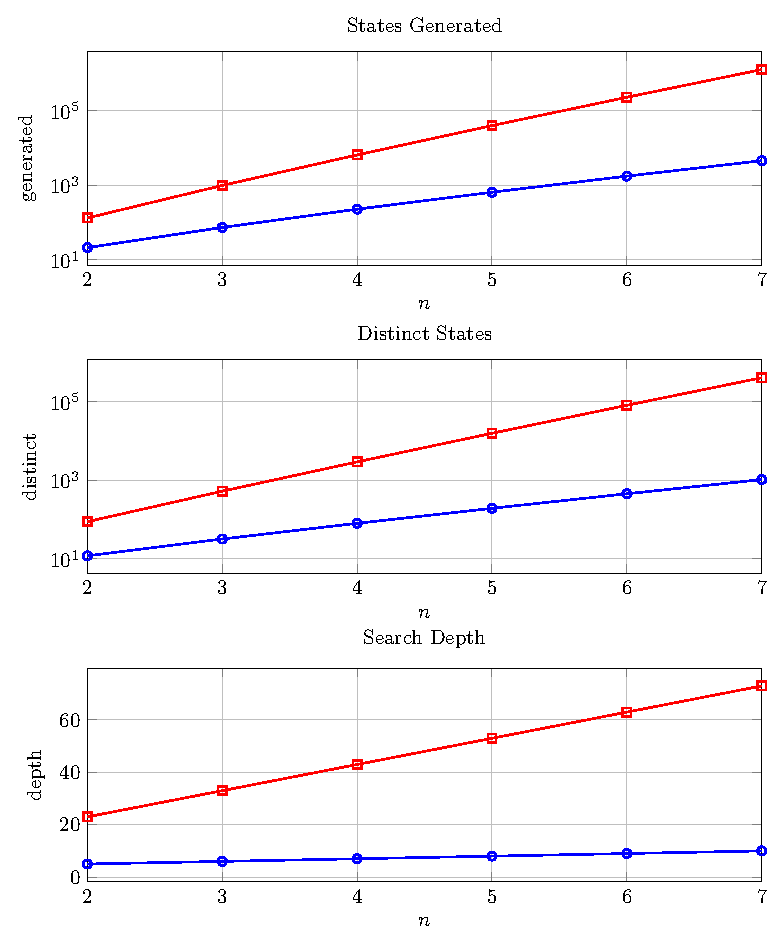
\includegraphics[width=0.88\textwidth]{results/plots/state_growth_plots.pdf}
\caption{Baseline 与 Udding 在 states generated、distinct states 和 search depth 上的增长趋势。}
\end{figure}

\begin{figure}[H]
\centering
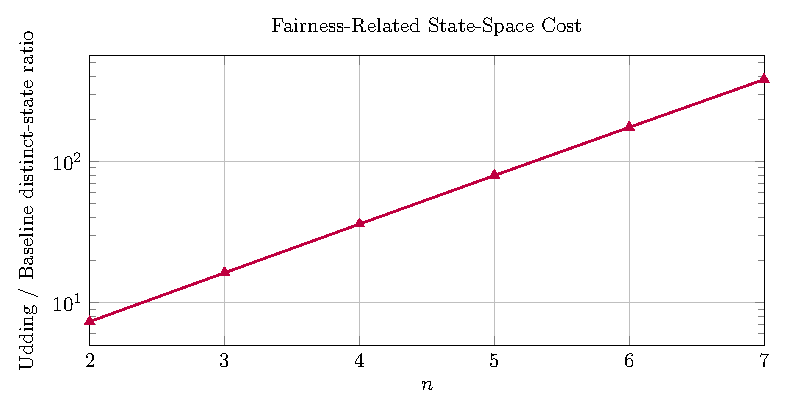
\includegraphics[width=0.72\textwidth]{results/plots/distinct_ratio_plot.pdf}
\caption{Udding 相对于 baseline 的 distinct-state ratio，用于刻画 fairness-related structure 带来的状态空间代价。}
\end{figure}

\subsection{Udding 的 fairness / no-starvation 结果}

在加入 \texttt{FairSpec} 和 \texttt{NoStarvation} 之后，我们对 Udding 模型进行的小规模 liveness 检查结果如下：

\begin{table}[H]
\centering
\caption{Udding 的 fairness-oriented liveness 检查结果}
\begin{tabular}{ccccc}
\toprule
$n$ & Specification & Property & Result & Time \\
\midrule
2 & \texttt{FairSpec} & \texttt{NoStarvation} & pass & 1 秒以内 \\
3 & \texttt{FairSpec} & \texttt{NoStarvation} & pass & 约 11 秒 \\
\bottomrule
\end{tabular}
\end{table}

这意味着当前 TLA+ 模型已经不仅仅能说明 Udding 的 safety 结构，也能够在显式 fairness assumptions 下，体现其原始算法设计中针对 starvation 的核心目标。

\section{对比与分析}

\subsection{两种协议都满足 safety}

对于 $n=2$ 到 $n=7$，baseline 和 Udding 都通过了 TLC 的 safety 检查。这说明两种协议都能满足最基本的 mutual exclusion 要求。

\subsection{真正的差别在于 fairness-related structure}

Baseline 的优势是结构最简单，状态空间增长也最温和。但它的简单来自于它根本不尝试约束“谁应该先被准入”。因此，在 weak fairness 条件下，它不能阻止等待者被反复超越。

Udding 则完全不同。它通过 \texttt{enter}、\texttt{queue}、\texttt{mutex}、\texttt{ne}、\texttt{nm} 把竞争拆分成多个阶段，使协议天然具有更强的 fairness-oriented structure。也正因如此，Udding 的额外复杂度不是无意义的开销，而是它为避免 starvation 所付出的结构性代价。

\subsection{公平性的状态空间代价}

最直观的量化结论是 Udding 与 baseline 之间的 distinct-state ratio：

\begin{table}[H]
\centering
\caption{Udding 相对于 baseline 的 distinct-state ratio}
\begin{tabular}{cccc}
\toprule
$n$ & Baseline Distinct & Udding Distinct & Ratio \\
\midrule
2 & 12 & 88 & 7.33x \\
3 & 32 & 520 & 16.25x \\
4 & 80 & 2880 & 36.00x \\
5 & 192 & 15264 & 79.50x \\
6 & 448 & 78208 & 174.57x \\
7 & 1024 & 390016 & 380.88x \\
\bottomrule
\end{tabular}
\end{table}

随着 $n$ 增长，这个比例上升得非常快。这清楚地说明：在 weak binary semaphore 前提下，如果我们希望协议更公平、更不容易让等待者饿死，那么形式化模型与验证代价都会显著上升。

\subsection{Peterson、baseline 与 Udding 的层次关系}

我们最终形成了一个清晰的层次：

\begin{itemize}
  \item Peterson 提供传统 mutual exclusion 的理论背景；
  \item 单 \texttt{mutex} weak-semaphore baseline 提供题目要求下的真正对照组；
  \item Udding 提供公平性导向的 semaphore 级协议解法。
\end{itemize}

这种组织方式也正好延续了 midterm 的思路：先说明最自然方案为什么不够，再说明为什么需要 Udding。

\section{公平性讨论}

公平性是本项目的核心主题。我们不试图证明 weak semaphore 自身是公平的；相反，我们承认底层原语只有弱公平能力。我们真正要说明的是：

\begin{itemize}
  \item baseline 展示了只保证互斥时协议可以有多简单；
  \item Udding 展示了当我们关心 overtaking 和 starvation 时，需要多少额外结构；
  \item 在显式 fairness assumptions 下，TLC 对 \texttt{NoStarvation} 的通过结果与 Udding 原论文的目标是一致的。
\end{itemize}

因此，之前做出的 $n=2..7$ 参数实验数据依然非常有价值。它们不仅说明协议是可扩展验证的，也量化了 fairness-related structure 的成本。新的 \texttt{NoStarvation} 结果则补上了“仅有 safety 还不够”的那一块。

\section{结论}

我们完成了 CE356 弱二元信号量项目的两个层面工作。第一，我们建立了 baseline 和 Udding 两个 TLA+ 模型，并对 $n=2$ 到 $n=7$ 做了系统的 safety 参数实验。第二，我们把 Udding 模型进一步扩展到 fairness-sensitive temporal checking，并在小规模上验证了 \texttt{NoStarvation}。

整个项目最重要的结论可以概括为：

\begin{quote}
在 weak binary semaphore 的约束下，获得 mutual exclusion 并不难，但想要获得更公平的准入行为，就必须付出显著更高的协议复杂度和验证成本。
\end{quote}

这也正是为什么 Udding 算法适合作为本项目的核心研究对象。

\appendix

\section{Baseline TLA+ 代码}
\lstinputlisting[language=TLA]{BaselineMutex_noComment.tla}

\section{Udding TLA+ 代码}
\lstinputlisting[language=TLA]{UddingMutex_noComment.tla}

\end{document}
